\documentclass[report,gutter=10mm,fore-edge=10mm,uplatex,dvipdfmx]{jlreq}

\usepackage{lmodern}
\usepackage{amssymb,amsmath}
\usepackage{ifxetex,ifluatex}
\usepackage{actuarialsymbol}
\usepackage[]{natbib}
\RequirePackage{plautopatch}

% maru suji ① etc.
\usepackage{tikz}
\newcommand{\cir}[1]{\tikz[baseline]{%
\node[anchor=base, draw, circle, inner sep=0, minimum width=1.2em]{#1};}}

\usepackage{comment}

\begin{comment}

\ifnum0\ifxetex1\fi\ifluatex1\fi=0 % if pdftex
  \usepackage[T1]{fontenc}
  \usepackage[utf8]{inputenc}
  \usepackage{textcomp} % provide euro and other symbols
\else % if luatex or xetex
  \usepackage{unicode-math}
  \defaultfontfeatures{Scale=MatchLowercase}
  \defaultfontfeatures[\rmfamily]{Ligatures=TeX,Scale=1}
\fi
% Use upquote if available, for straight quotes in verbatim environments
\IfFileExists{upquote.sty}{\usepackage{upquote}}{}
\IfFileExists{microtype.sty}{% use microtype if available
  \usepackage[]{microtype}
  \UseMicrotypeSet[protrusion]{basicmath} % disable protrusion for tt fonts
}{}
\makeatletter
\@ifundefined{KOMAClassName}{% if non-KOMA class
  \IfFileExists{parskip.sty}{%
    \usepackage{parskip}
  }{% else
    \setlength{\parindent}{0pt}
    \setlength{\parskip}{6pt plus 2pt minus 1pt}}
}{% if KOMA class
  \KOMAoptions{parskip=half}}
\makeatother
\usepackage{xcolor}
\IfFileExists{xurl.sty}{\usepackage{xurl}}{} % add URL line breaks if available
\IfFileExists{bookmark.sty}{\usepackage{bookmark}}{\usepackage{hyperref}}
\hypersetup{
  hidelinks,
  pdfcreator={LaTeX via pandoc}}
\urlstyle{same} % disable monospaced font for URLs
\usepackage{longtable,booktabs}
% Correct order of tables after \paragraph or \subparagraph
\usepackage{etoolbox}
\makeatletter
\patchcmd\longtable{\par}{\if@noskipsec\mbox{}\fi\par}{}{}
\makeatother
% Allow footnotes in longtable head/foot
\IfFileExists{footnotehyper.sty}{\usepackage{footnotehyper}}{\usepackage{footnote}}

\end{comment}
%\makesavenoteenv{longtable}
\setlength{\emergencystretch}{3em} % prevent overfull lines
\providecommand{\tightlist}{%
  \setlength{\itemsep}{0pt}\setlength{\parskip}{0pt}}
\setcounter{secnumdepth}{-\maxdimen} % remove section numbering

\author{kazuyoshi}
\date{}

\newcommand{\problem}[1]{\subsubsection{#1}\setcounter{equation}{0}}
%\newcommand{\answer}[1]{\subsubsection{#1}}
\newcommand{\answer}[1]{\subsubsection{解答}}

%Pdf%\newcommand{\wakumaru}[1]{\framebox[3zw]{#1}}
\newcommand{\wakumaru}[1]{#1}





\begin{document}
\chapter{保険1第5章 変額年金保険}
\section{5.1 変額年金保険の概要}
\problem{H27 生保1問題 2(2)①}
変額年金保険の最低保証のバリエーションである「ラチェット型」と「ノックアウト型」について簡
潔に説明しなさい。なお、保険会社の収益に与える影響についても言及すること。
\answer{}

「ラチェット型」\\
・運用実績が好調で特別勘定の積立金が一定水準を上回れば、その度に最低保証額が切りあがっ
ていき(ラチェットアップ)、その後運用実績が悪化しても最低保証額は下がらない方式。\\
・オプション価値を引き上げる効果を持ち、保険会社にとっては、特別勘定の運用実績が良好な
場合の解約の抑止すなわち保険関係費用収入の増加効果もある。

「ノックアウト型」\\
・特別勘定残高の目標水準超過あるいは下限(フロア)抵触で、自動的に特別勘定から一般勘定に
全部または一部の金額をキャッシュアウトし、オプションが消滅する方式。\\
・オプション価値を引き下げる効果がある一方で、保険会社にとっては、特別勘定での滞留時間
が減ることから保険関係費用収入の減少効果もある。

\section{5.2 最低保証リスクの基本的構造}
\problem{H28 生保 1 問題 1(3)}
変額年金保険の最低保証リスクの基本的構造に関する以下の説明に関し、次の①~⑤に適切な語句を
記入しなさい。\vspace{1zh}

変額年金保険のもつリスク特性は、伝統的な生命保険とは大きく異なる。一般的な変額年金保険で
は、保険会社には契約者の運用資産である投資信託を管理する特別勘定と最低保証機能を担う一般勘
定の機能が同時に求められる。一般勘定の引受リスクは最低保証した金額と特別勘定残高の差額であ
り、保証された保険金を行使価格とする「保険関係費用+運用関係費用相当の外部流出のある原資産の
\wakumaru{①}」を販売していることに相当する。

被保険者の生死を条件としない満期保証は一部の投資信託でも見られ、最も単純なものは満期保証
額をカバーできるような割引債と超過収益獲得のための\wakumaru{②}を組み合わせる形式がとられるが、
変額年金保険の最低保証では、保証機能のない通常の投資信託と保険会社の引き受ける
\wakumaru{①}による構成が一般的である。
\wakumaru{③}・オプションの\wakumaru{④}から、両者は契約時点では等価であることは自明で
あるが、こういったオプションが一般的には取引されておらず何らかの複製手法によらざるをえない
ため、少なくとも\wakumaru{⑤}
リスク管理に関しては、多くの部分を割引債で静態的にヘッジできる前者の
リスク管理負荷がより小さく、商品の供給サイドにとっては有利である。
\answer{}
\begin{itemize}
\item[①: ] プット・オプション
\item[②: ]コール・オプション
\item[③: ] ヨーロピアン
\item[④: ] プット・コール・パリティ
\item[⑤: ]金利
\end{itemize}

\problem{H24 生保 2 問題 2(4)}
変額年金保険における最低保証の金融リスクおよび保険リスクについて、簡潔に説明しなさい。
\answer{}
<最低保証の金融リスク>\\
一般的な変額年金保険では、保険会社には契約者の運用資産である投資信託を管理する特別勘
定と最低保証機能を担う一般勘定の機能が同時に求められる。一般勘定の引受リスクは最低保
証した金額と特別勘定残高の差額であり、保証された保険金を行使価格とする「保険関係費用
(最低保証料と予定事業費)+運用関係費用(信託報酬等)相当の外部流出のある原資産のプ
ットオプション」を販売していることに相当する。\\
一般にオプションの原資産である投資信託の運用に保険会社は関与せず、契約者が投信の資産
配分の変更を指示できるものも存在する。また、投資信託に対応するヘッジ手段が必ずしも市
場で購入可能とはいえないため、一般的な金融商品に比べリスクコントロールの負荷は大き
い。\\
また、オプション料に相当する最低保証料は特別勘定資産の残高比例で日々徴収されることが
一般的であるため、特別勘定資産が減少し最低保証の本源的価値が高まるほど最低保証料収入
が減少し、特別勘定資産が増加し最低保証の本源的価値が低下するほど最低保証料収入が増加
するというミスマッチ構造を有している。そのため、保険料収入の一部を内部留保して将来の
リスクに備えるという伝統的な保険数理の考え方だけではリスクコントロールがうまく機能し
ない可能性がある。\\
さらに、最低保証オプションは、その長期性と原資産が投資信託という特殊性から、市場で一
般的に取引されるデリバティブでの複製は難しい。また、オプションの単価に影響する金融リ
スクと、契約の残存量に対応しオプションの数量に影響する死亡や解約といった保険リスクの
積の構造をもつため、金融市場での完全な複製は困難である。

<最低保証の保険リスク>\\
伝統的な生命保険数理では被保険者の生死を生命表に従う決定論的なモデルとして取り扱って
きたが、これは各被保険者の死亡事象が独立としたときに被保険者数を増やすことでリスクが
収斂していくことに依存している。変額年金保険の保険数理の実務においても、被保険者の生
死に関するモデリングは生命表と生命関数を用いた伝統的な生命保険数理の考えに従うものと
なっているが、変額年金保険では特別勘定を原資産とするオプションのペイオフに対応する金
融リスクが共通に関与するため、被保険者数増加によるリスクの収斂性は伝統的な保険よりも
劣後する。\\
実際には、年齢・性別を問わない「一律の最低保証料率(保険関係費用率)」や
「職業のみによる危険選択」など、保険リスクに関してアグレッシブなものとなっている。
この問題はオプションの満期の平均的な長さの違いやオプション料の収入現価の多寡に直結するため、
金融リスク面でもミスプライスの要因となりうる。\\
さらに、死亡率以上に大きな影響をもつ保険リスクファクターが解約率である。実務では、非
合理的な解約行動を織り込んで、何らかの統計的推定に基づき経過時間や、原資産価格と保証
水準の関係等に応じた決定論的なモデルが用いられることが多いが、販売開始からの期間も短
く、商品性も多様であるため解約率モデルのベースとなる統計が死亡率ほど頑健なものとはい
えない。
\section{5.3 変額年金保険数理の基本的考え方}
\problem{2022 生保1問題 1(4)}
変額年金保険について、次の①~④に適切な語句を記入しなさい。(4点)\footnote{後半は 5.5 リスク管理 とヘッジの内容である}

プライシングの基本的な考え方として、変額年金保険における保険料(保険料比例の予定事業費
を徴収しないものとする)は\wakumaru{①}
投入額を意味する名目的なものにすぎないので、変額年金
固有のプライシングの論点は保険関係費用率、特に最低保証費用率の設定にある。

保険関係費用率のうち最低保証費用率は基礎書類記載事項であるが、予定事業費率(の水準)は
各社の内規によることとされており、事後的に実際の事業費と比較したモニタリングが求められる。
ただし、最低保証費用率の算出には、\wakumaru{①}
からの控除費用率全体を確定させる必要があり保
険関係費用率も必要になるので、現実にはこれらは同時決定される。
\vspace{1zh}

リスク管理に関して、変額年金保険の最低保証の金融市場での完全なヘッジは困難であるが、部
分的でもヘッジを行うことは考えられる。流動性の高いヘッジ手段と
\wakumaru{②}の間のずれ(ベー
シス・リスク)があるのは普通であって、ずれを計算に入れた適切な割合でヘッジを行うことが求
められる。

最低保証のリスクをいかに評価するかということは、ヘッジに対する考え方とも綿密に関係して
いる。最低保証のヘッジの目的としては
\begin{itemize}
\item[ A.]  経済価値のヘッジ、
\item[ B.]  会計価値のヘッジ、
\item[ C.]  AまたはBの\wakumaru{③}リスクのヘッジ
\end{itemize}
という3パターンが想定される。

\wakumaru{③}
リスクのヘッジは株価の大幅下落等の
\wakumaru{③}
イベントにおける最低保証の損失
によって最低保証に対応する資本が枯渇しないことを目的とする。
この場合、
\wakumaru{④}
ザマネーのプットオプションの買い持ちによる静態的ヘッジが想定され、
\wakumaru{④}
ザマネーであるため比較的ローコストで済むというメリットがある。

\answer{}
\begin{itemize}
\item[ ① : ] 特別勘定 
\item[ ② : ] ヘッジ対象 
\item[ ③ : ] テイル 
\item[ ④ : ] アウトオブ
\end{itemize}

\problem{2020 生保1問題 1(4)}
CTEの多期間適用時の問題点について、次の①~⑤に適切な語句または数値を記入しなさい。
①〜④の解答は、小数点以下第1位を四捨五入して整数で記入しなさい。

2期間の二項モデル(原資産の価格上昇確率:Pu=93%、同下落確率:Pd=7%)を考え(時
点0、1は保険金支払までに到来する決算期である)、時点2においてのみ各ノードで以下の保険金
支払があるものとする。\\
\hspace{3zw}(uu)=0,(ud)=60,(du)=0,(dd)=100

なお、『(X)』は、記号Xを価格上昇uまたは価格下落dのいずれかをとるものとした場合に、時点
1でXとなるノードを示す。
『(XY)』は、記号X,Yを価格上昇uまたは価格下落dのいずれかをと
るものとした場合に、時点1でX、時点2でYとなるノードを示す。\vspace{1zh}

このとき、各ノードにおける信頼区間95%のCTEは、下表のとおりとなる。

\begin{tabular}{|c|c|c|}
\hline
時点0& 時点1 & 時点2\\ \hline
 \multirow{4}{*}{CTE=\wakumaru{①}} & \multirow{2}{*}{(u) CTE=\wakumaru{②}}&(uu) 0\\ \cline{3-3}
 & & (ud) 60\\  \cline{2-3}
 & \multirow{2}{*}{(d) CTE=\wakumaru{③}}& (du) 0\\ \cline{3-3}
&&(ud) 100\\  \cline{1-3}
\end{tabular}

\vspace{1zh}
ここで、当該保険負債のみを保有し、時点0、時点1での責任準備金およびソルベンシー・マージ
ンの積立を信頼区間95%のCTEで要請し、時点0において、要請どおりの責任準備金およびソル
ベンシー・マージンの積立を行った保険会社を考える。

時点0における信頼区間95%のVaRは\wakumaru{④}
で、積立額(CTE)はこれより大きいことから、
時点0において破綻確率5%未満の安全性が確保されているはずである。

しかしながら、時点1でノード(d)に至った場合には
\wakumaru{③}
の資金が必要になり、当該保険会社
は破綻するが、その破綻確率は7%であることから、破綻確率5%未満の前提と矛盾する。

この問題点は\wakumaru{⑤}
の欠如と呼ばれている。
\answer{}
\begin{itemize}
\item[ ① ]  64 
\item[ ② ]  60 
\item[ ③ ]  100 
\item[ ④ ]  60 
\item[ ⑤ ]  通時一貫性
\end{itemize}

\problem{H25 生保1問題 1(5)}
VaR と CTE について簡潔に説明した上で、それぞれの特徴を説明しなさい。なお、VaR と CTE の
説明にあたっては、数式で説明することも可とする。
\answer{}
VaR・CTE の説明

数式の場合\footnote{公式解答と教科書の通り. 損保数理で習った定義と違うように見えるので注意}:\par  
VaR(α)=inf \{ x∈R:F(x)≧1-α\}\par
CTE(α)=E[X\textbar {VaR(α) ≧ X ]

文章の場合:\par
VaR は、ある一定の確率の範囲内(信頼区間)でどの程度の損失が発生する可能性
があるかを表す指標であり、例えば VaR99\%が 100 億円の損失とは 99\%の確率で
損失は 100 億円以下に抑えられるということである。\par 
一方で、CTE は信頼区間を
超える部分の期待損失であり、例えば CTE95\%が 100 億円の損失とは、損失が大
きい上位 5\%の期待値を取ると 100 億円の損失となるということである。

VaR・CTE の特徴\\
・VaR は直観的な把握が容易で扱いやすい。\\
・VaR は信頼区間外のリスクの規模を把握できないためテイルの長いリスクの把握に向かない。\\
(・一方で、CTE はテイルの長いリスクの把握も可能である。)\\
・VaR は凸性を満たさないことから分散効果の把握に潜在的弱点がある。\\
(・一方で、CTE は凸性を満たすコヒーレントリスク尺度である。)\\
・CTE は通時一貫性がないため、多期間のリスク尺度として使用する場合、問題点が生じる。

\problem{H21 生保 2 問題 2(1)}
変額年金保険の最低保証部分の責任準備金等を評価するためのアプローチである、CTEアプローチ
とリスク調整済み期待値アプローチについて、簡潔に説明しなさい。
\answer{}
最低保証部分の給付額は特別勘定積立金額の増減に対して対称ではなく、一種の金融オプションで
あることから、従前の商品に用いていた大数の法則を前提とした決定論的な手法では十分な責任準備
金評価が行えない。そこで、特別勘定の原資産価額変動を確率的にとらえ、金融リスク管理の手法を
とりいれた責任準備金の評価方法が必要となり、その方法の計算原理として、CTEアプローチおよび
リスク調整済み期待値アプローチがある。\\
CTEアプローチ

CTEアプローチとは、確率分布の一部(テイル)の期待値を用いるものであり、分位原理の一種で
ある。具体的には、信頼水準αに対して、責任準備金が増大する悪化事象の下方α分位までの条件付
期待値CTE(α)をもって評価する。

コヒーレント・リスク尺度であるが、冬期間のリスク尺度としては通時一貫性がないなどの欠点が
ある。

カナダ等の変額年金保険規制において、最低継続自己資本規制・最低資本準備金算出に用いられて
いる。\\
リスク調整済み期待値アプローチ

リスク調整済み期待値アプローチは確率分布全体を使い、その期待値をもって評価する期待値原理
の一種である。確率分布が同じであればCTE(0%)と同じ結果となるが、リスク調整済み期待値ア
ブローチでは、オプション評価のような無裁定価格導出のためのリスク中立測度を含む、リスク調整
に相当する測度変換後の確率分布の下で期待値をとる。

CTEの通時一貫性がないという問題が回避可能となる。ただし、真の市場整合的評価に近づけるに
は、金利の期間構造や、オプション期間とインザマネーの度合いに応じたインプライド・ボラティリ
ティーの違いの反映等が必要となるが、モデルとパラメータの内製化のハードルは極めて高いといっ
た難点がある。

日本の標準的方法は、計量化の手段はVaRであるが、期待収益率および現価計算の割引率に標準
利率を用いる点で、リスク調整済みアプローチの考え方を採用している。\\
※上記の他、次の点に触れている場合加点した。\vspace{1zh}

CTE\\
最低保証の価値評価と必要資本要件のためのリスク評価を同じCTEの枠組で行うことができる。\\
悪化シナリオにもとづいて評価する方式自体に保守性が組み込まれているため、原資産の変動を
表現するためのパラメータは必ずしも保守的に設定する必要はない。\\
テイル表現能力を重視した原資産収益率モデルが必要。

リスク調整済み期待値アプローチ\\
リスク調整は価値評価のためだけのもので、必要資本要件のためのリスク評価は、原資産価格変
動やモデル・パラメータの変動がこの価値の変動に与える影響幅を所定の信頼水準で見るといっ
た、別の枠組を用いる。\\
評価方式自体には保守性が組み込まれていないため、責任準備金を保守的に評価するためには基
確率を保守的に設定する必要がある。\\

ファットテイルの影響:CTEアプローチに対してリスク調整済み期待値アプローチは影響を受けに
くい。

シナリオテスト(シミュレーション)でのシナリオ数:安定した結果を得るのに、CTEアプローチに
対してリスク調整済み期待値アプローチは比較的少なくて済む。
\section{5.4 変額年金保険数理の法定実務}
\subsection{最低保証に係る保険料積立金計算の概要}
\problem{2020 生保2問題 1(6)}
変額年金保険等の最低保証に係る保険料積立金の積立てに際して予定解約率を使用する場合の留
意点について、保険会社向けの総合的な監督指針の記載を踏まえ、簡潔に説明しなさい。
\answer{}
\begin{itemize}
\item[]  予定解約率が過去の実績や商品性等から、合理的に定められたものとなっているか。
\item[]  例えば、以下の事例等に留意しているか。
\begin{itemize}
\item[]  特別勘定の残高が最低保証額を下回る状態にあるときの解約率が、特別勘定の残高が最低保証額を超える状態にあるときの解約率より低い率となっているか。
\item[]  解約控除期間における解約率が、解約控除期間終了後の解約率と比べ、低い率となっているか。
\item[]  最低年金原資保証が付された保険契約で、年金開始前における特別勘定の残高が最低保証額を下回る状態にある場合において解約率を保守的に設定しているか。
\item[]  設定された予定解約率について、解約実績との比較などにより、検証を行うこととなっているか。
\end{itemize}
\end{itemize}

\problem{H26 生保2問題 1(3)}
変額年金保険の最低保証に係る保険料積立金について、次の空欄を埋めなさい。

標準的方式の考え方としては、 「一般勘定における最低保証に係る保険金等の支出現価から一般
勘定における最低保証に係る純保険料の収入現価を控除する形式の計算式」によって概ね
\wakumaru{①}%以上の事象をカバーできる水準とされている。この水準は、
\wakumaru{②}アプローチで特にリスク中立評価を意識したものと解釈できる。

標準的方式では、 計算式表現によることが要件とされているが、 商品が複雑な場合等は近似的
な計算式も可とされている。ただし、同じ近似法でも\wakumaru{③}
を用いた場合は、モデルや基礎率如何にかかわらず標準的方式とは認められない。

代替的方式では、 標準的方式と同じ期待収益率と
\wakumaru{④}を使う場合を除き、 代替的方式で計算
される保険料積立金の額が、期待収益率と
\wakumaru{④}以外の代替的方式の基礎率を標準的方式に反映して計算される額と
\wakumaru{⑤}%以上乖離しないことの確認が求められている。
\answer{}
\begin{itemize}
 \item[①: ]  50
 \item[②: ]  リスク調整済み期待値
 \item[③: ]  モンテカルロ法
 \item[④: ]  ボラティリティー
 \item[⑤: ]  10
\end{itemize}

\problem{H23 生保 2 問題 1(2)}
変額年金保険等の最低保証に係る保険料積立金に関し、以下の①~⑤の空欄に当てはまる適切な語
句を記入しなさい。

保険料積立金の積立てに際して予定解約率を使用する場合には、標準的方式か代替的方式かを問わ
ず\wakumaru{①}および\wakumaru{②}から合理的とみなされる解約率の使用が認められているが、次の4要件が「保
険会社向けの総合的な監督指針」で要請されている。

\wakumaru{③}が最低保証額を下回る状態にあるときの解約率は、
\wakumaru{③}が最低保証額を超える状態にあるときの解約率より低いこと。

\wakumaru{④}における解約率が、\wakumaru{④}終了後の解約率より低いこと。

\wakumaru{⑤}が付された保険契約で、年金開始前における\wakumaru{③}
が最低保証額を下回る状態にある場合において解約率が保守的に設定されていること。

解約実績との比較などにより検証を行うこと。

\answer{}
\begin{itemize}
\item[①: ] 過去の実績
\item[②: ] 商品性
\item[③: ] 特別勘定の残高
\item[④: ] 解約控除期間
\item[⑤: ] 最低年金原資保証
\end{itemize}

\problem{H18 生保2問題 2(1)}

平成 8 年・大蔵省告示第 48 号第 5 項に規定されている、変額年金保険等の最低保証に係る保険料積
立金の積立方式である「標準的方式」を簡潔に説明せよ。また、それを使用する場合における留意点を
挙げ、金融庁の「保険会社向けの総合的な監督指針」の記載内容を踏まえ簡潔に説明せよ。
H17 生保2問題 2(2) (範囲外:テキストより削除済み)
平成 17 年度から導入された危険準備金Ⅲの対象とするリスク、積立基準、積立限度、取崩基準およ
び平成 17 年度の経過措置について、簡潔に説明せよ。

\answer{}
<「標準的方式」の内容について>

「標準的方式」により計算される保険料積立金は次の①から②を控除した金額である。\\
①一般勘定における最低保証に係る保険金等の支出現価\\
②一般勘定における最低保証に係る純保険料の収入現価

<「標準的方式」を使用する場合における留意点>

[全般]: 通常予測されるリスクに対応するものとして、標準的な計算式によって、概ね
50%の事象をカバーできる水準に対応する額を算出するものとする。

[予定死亡率]: 最低死亡保険金保証が付された保険契約においては死亡保険用の標準死
亡率を、最低年金原資保証が付された保険契約については年金開始後用の標準死亡率を、
両方の保証が付された保険契約においては、保険料積立金の積立が保守的となる方の標
準死亡率を使用する。

[割引率]: 割引率として標準利率を使用する。

[期待収益率]: 期待収益率として標準利率を使用する。

[ボラティリティ]: 資産種類に応じて以下のボラティリティを使用する。なお、下記以
外の資産種類のボラティリティに関しては過去の実績等から合理的に定めたものを使
用する。\\
国内株式:18.4%、邦貨建債券:3.5%、\\
外国株式:18.1%、外貨建債券:12.1%

[予定解約率]: 以下の点に留意したうえで、過去の実績や商品性等から合理的に定める。\\
特別勘定の残高が最低保証額を下回る状態にあるときの解約率が、特別勘定の残高
が最低保証額を超える状態にあるときの解約率より低い率とする。\\
解約控除期間における解約率が、解約控除期間終了後の解約率と比べ、低い率とする。\\
最低年金原資保証が付された保険契約で、年金開始前における特別勘定の残高が最
低保証額を下回る状態にある場合において解約率を保守的に設定する。\\
設定した予定解約率について、解約実績との比較などにより、検証を行う。

[その他の基礎率]: 過去の実績や商品性等から合理的に設定する。

\subsection{ソルベンシー・マージン基準の最低保証リスク計算の概要}
\problem{H27 生保 2 問題 1(5)}
平成 8 年・大蔵省告示第 50 号別表第 6 の 2 に規定されている、変額年金保険等の最低保証リスク相
当額の算出について、次の A~E に適切な語句を記入しなさい。\\
Ⅱ.最低保証リスク相当額の算出\\
1.標準的方式\\
(1) 最低保証リスク相当額は、次のイに掲げる額からロに掲げる額を控除した額とする。

イ \wakumaru{A} 責任準備金の額(原則として法第 4 条第 2 項第 4 号に掲げる書類に記載された商品区分
ごとに、次の①から④までに定める手順に基づき算出した額をいう。)

① 次に掲げる区分に応じたリスク対象資産の額から、別表第 7 の 2 の区分によるそれぞれの対
象取引残高の欄に掲げる額(別表第 7 の 2 によりリスクヘッジの有効性が確認できたものに
限る。)を控除した残高に、次の表に掲げる区分に応じた下落率をそれぞれ乗じた額の合計額
を算出する。(省略)

② 上記①に掲げる額から、その額に次に掲げる算式により計算した\wakumaru{B}係数を乗じた額を控除
する。(省略)

③ 上記②により算出した額を特別勘定資産の額の合計額で除した率を算出する。

④ 上記③により算出した率に基づき資産下落が生じたとした場合の、一般勘定における
\wakumaru{C}の額を算出する。

口 法第 4 条第 2 項第 4 号に掲げる書類に記載された方法に基づき算出された一般勘定における
\wakumaru{C}の額

(2) (省略)

(3) (省略)\\
2.代替的方式

次の①から⑬に定める基準を満たす保険会社、外国保険会社等又は免許特定法人(以下「保険会社
等」という。)は代替的方式を用いることができる。ただし、代替的方式を用いた場合は、
\wakumaru{D}の結果、
代替的方式の使用を継続することが不適当と認められ、代替的方式の使用を中断する旨又は
\wakumaru{E}に重大な変更を加える旨をあらかじめ金融庁長官に届け出た場合を除き、これを継続して使用
しなければならない。

(以下、省略)
\answer{}
\begin{itemize}
 \item[A: ] 資産価格下落後
 \item[B: ] 分散投資効果
 \item[C: ] 最低保証に係る責任準備金
 \item[D: ] バック・テスティング
 \item[E: ] リスク計測モデル
\end{itemize}
\subsection{その他留意事項}
\problem{2021 生保2問題 1(2)}
変額年金保険の利源分析について、以下の①~⑤の空欄に当てはまる適切な語句を記入しなさい。

金融庁提出用の決算状況表記載の利源分析(6利源への分解)では、最低保証に係る保険料積
立金の積み立て・取り崩しは\wakumaru{①}
で認識する。なお、発生要因が対象資産の価値の変動で
あることに鑑みれば、内部管理としては\wakumaru{②}として認識することも考えられる。

また、金融庁提出用の決算状況表記載の利源分析では、保険料積立金を
\wakumaru{③}式で計上する一方で、危険差(死差)損益中の予定事業費は
\wakumaru{④}式で表示されるため、そのままでは
危険差損益が歪んでしまう。このため、
\wakumaru{④}式と\wakumaru{③}式の予定事業費の差額(これを\wakumaru{⑤}
という)を危険差損益の貸方に計上して危険差の歪みを回避しつつ、
借方に同額を計上して全体としては貸借が相殺されるような調整を行う。

\answer{}
\begin{itemize}
\item[ ①: ] 責任準備金関係損益
\item[ ②: ] 価格変動損益
\item[ ③: ] 純保険料
\item[ ④: ] 5年チルメル
\item[ ⑤: ] 予定事業費調整 (「予定事業費修正」も可。)
\end{itemize}

\problem{H29 生保1問題 1(2)}
変額年金保険に関連する次の①~⑤の記述について、下線部分が正しい場合は○を記入し、誤っ
ている場合は×を記入するとともに下線部分を正しい内容に改めなさい。

① 「オプション価格の原資産ボラティリティーに対する感応度」のことを \underline{Vega} と呼ぶ。

② リスク尺度$\rho$がコヒーレントであるためには、
「確率変数 X が、
任意の実数$\lambda>0$ に対して、
『$\rho(\lambda X)=\lambda\rho(X)$』である。」という性質を満たしていることが必要であるが、
この性質を\underline{定数不変性}という。

③ 最低保証のある変額年金保険等は、毎年、最低保証に係る収支残以上の金額を危険準備金Ⅲに積み
立てることとされるが、その上限は保険料積立金(一般勘定の最低保証に係わるものと特別勘定に
係わるもの)の \underline{5\%}である。

④ 最低保証に係る保険料積立金の標準的方式の考え方としては、「一般勘定における最低保証に係る
保険金等の支出現価から一般勘定における最低保証に係る純保険料の収入現価を控除する形式の
計算式」
(標準的な計算式)によって概ね \underline{95%}以上の事象をカバーできる水準とされる。

⑤ 保険会社向けの総合的な監督指針において、最低保証に係る保険料積立金の計算で予定解約率を使
用する場合、「\underline{保険料払込}期間における解約率が当該期間終了後の解約率と比べて低い率となって
いるか」等に留意することとされる。
\answer{}
\begin{itemize}
\item[①: ]  ○
\item[②: ]  × 正同次性
\item[③: ]  × 6%
\item[④: ]  × 50%
\item[⑤: ]  × 解約控除
\end{itemize}

リスクパラメータ (Greeks)\\
Delta: 原資産価格に対する感応度\\
Gamma: Deltaの感応度\\
Vega: 原資産ボラティリティーに対する感応度\\
Rho: 金利に対する感応度

\section{5.5 リスク管理とヘッジ}
\subsection{経済価値のヘッジ、会計価値(責任準備金)のヘッジ}
\problem{H26 生保1問題 1(5)}
変額年金保険の最低保証リスクにおける会計価値のヘッジについて、その概要を簡潔に説明しなさ
い。また、この会計価値のヘッジは経済価値のヘッジに比べ困難な点があるが、その理由を簡潔に説
明しなさい。
\answer{}
会計価値のヘッジとは、貸借対照表上の純資産の変動や、損益計算書上の損益の変動をコント
ロールすることを目的とするヘッジのことである。

最低保証リスクのヘッジには、通常はデリバティブが用いられるが、デリバティブは会計上時
価評価される。一方、会計上の負債(責任準備金)は時価評価されない。このため、ヘッジ資
産の評価とのミスマッチが生じやすい。

具体的には、最低保証のための責任準備金は負値をとらないことや、その評価に用いる金利(標
準利率)やボラティリティーが固定(ロック・イン)されていることが、ミスマッチの要因と
して挙げられる。

\problem{H23 生保 1 問題 2(2)}
変額年金保険の最低保証における「経済価値のヘッジ」と「会計価値のヘッジ」のそれぞれの概要
について、両者の目的の違いを踏まえたうえで簡潔に説明しなさい。
\answer{}
変額年金保険の最低保証における「経済価値のヘッジ」と「会計価値のヘッジ」は、ヘッジの対象
となる最低保証の価値について、経済価値で評価した負債を用いるか、あるいは会計上の負債(責任
準備金)を用いるか、という点で異なっている。

経済価値のヘッジは、デリバティブによる負債の経済価値の複製とそれによるリスクの中和を意図
しており、経済価値の変動の抑制を目的としている。ヘッジ手法としては、原資産価格に対応する感
応度であるDelta,Deltaの感応度であるGa㎜a、原資産ボラティリティの感応度であるVega、金利
の感応度であるRhoといったリスクパラメータに分解し、Deltaに対しては主に先物を、Ga㎜aやVega
は主にオプションを、Rhoは主に金利スワップを用いる等、リスクパラメータに応じたヘッジ手法を
用いる。また、比較的短期でロールが必要な先物等を用いた動態ヘッジと長期のオプションの買い持
ちによる静態ヘッジ、あるいはその混合がある。なお、経済価値のヘッジは、解約等のモデルリスク
等により完全なヘッジは困難が伴うことや、負債が時価評価されない会計とはミスマッチが生じる等
の課題がある。

会計価値のヘッジは、会計的価値の変動を抑制することを目的としているが、一般的に、責任準備
金は制度上負の値を取らないこと、責任準備金の基礎率は金融市場のパラメータと構造・水準が一致
しないこと等から、デリバティブによる負債価値の複製は困難である。また、最低保証の責任準備金
の基礎率がロックインされ、金利やボラティリティが固定されることから、先物以外のヘッジは使い
づらいこととなる。

\problem{2019 生保 1 問題 1(6)}
変額年金保険の最低保証リスクにおける経済価値ヘッジのうち、Delta ヘッジについて、仕組
みを簡潔に説明した上で、その留意すべき弱点を挙げなさい。
\answer{}

[仕組み]\\
経済価値のヘッジは、デリバティブでの経済価値の複製により、リスクの中和を図ることで
ある。特に Delta ヘッジは、原資産価格に対するオプション価格の感応度である Delta を把
握し、これを打ち消す Delta をデリバティブで複製し、リスクの中和を図ることである。\\
Delta の複製には、先物を現物のポジションに合わせて短期間で調整していくことが一般的で
ある。

[留意すべき弱点]\\
短期のヘッジを長期に亘って短期の調整を繰り返していくのに負荷がかかる。\\
微小な価格変動にしか有効でないため、市場環境が大きく変化した場合に追随できない。\\
金利水準の変化に対応できない

\subsection{具体的なヘッジ手法}
\problem{H27 生保 1 問題 2(2)②}
最低保証リスクのヘッジにおいて、デリバティブ・再保険を用いる際の留意点をそれぞれ簡潔に説明
しなさい。
\answer{}

「デリバティブ」\\
最低保証の保険期間に対応するような長期のデリバティブ市場は薄く、最低保証の対象となる
すべての原資産に対して先物やデリバティブが利用できるわけではない。また、ヘッジには誤
差がつきものであり、モデルエラーやトラッキングエラーは不可避であるが、特に最低保証の
場合は解約率モデルの影響が大きく、実績と見通しのズレにより大きなオーバーヘッジ、アン
ダーヘッジが発生しうることに留意する必要がある。
その他、管理に際しインフラ等にコストがかかること、ヘッジコストはマーケット環境等によ
り変動すること、カウンターパーティーリスクの管理等にも留意する必要がある。

「再保険」\\
再保険により、会計とのバッティングなしにリスクヘッジするには、責任準備金の削減が可能
な(修正)共同保険式再保険が適しており、再保険会社の信用リスク管理や集中リスクを回避
する等の対策、再保険料はマーケット環境等により変動すること等に留意する必要がある。

\section{ノート(1~7)}
\subsection{<ノート4>カナダにおける株式のテイル・モデリング}
\problem{H23 生保 1 問題 1(1)}

局面転換対数正規モデル(RSLN2)による株価収益率モデルとして次のようなモデルが構成されて
いる。
\begin{itemize}
\item $S_t$ :第$t$期における特別勘定資産価値
\item $LN(\mu_1,\sigma^2_1)$:局面1の対数正規分布
\item $LN(\mu_2,\sigma^2_2)$:局面2の対数正規分布
\item $\begin{pmatrix}
 1 - p_{12} & p_{12} \\
 p_{21} & 1 - p_{21}
 \end{pmatrix}$ :局面間の推移確率行列、$p_{ij}$は局面$i$から局面$j$への推移確率
\end{itemize}

このとき、定常状態を想定して局面1にある確率 $\pi_{1}$ を求めると\\
$\pi_1$ = [ ① ](算式表示)である。\\
また、
$\begin{pmatrix}
1 - p_{12} & p_{12} \\
p_{21} & 1 - p_{21}
\end{pmatrix}
=
\begin{pmatrix}
0.9 &0.1 \\
0.2 & 0.8
\end{pmatrix}$
とすると、局面2にある確率$\pi_2$は
$\pi_2$ = [ ② ](分数表示)となる。

一様乱数により初期局面(第0期)をシミュレーションすると、初期局面は局面1であった。
標準正規乱数を $z_0$ とすると、第1期の資産価値は
$S_1=S_0\times$ [ ③ ](算式表示)となる。

ここで、標準正規乱数を発生させ、$z_0$ = 0.03297を取得した。

$ \mu_1= 0.012, \sigma_1 = 0.035, \mu_2 = -0.016, \sigma_2 = 0.078$

であるとき、$\log{\frac{s_1}{s_0}}$=[ ④ ](小数点以下第6位を四捨五入)となる。

さらに、シミュレーションを継続し、乱数を発生させた結果は次のとおりであった。

\begin{tabular}{|c|c|c|c|c|}
\hline 第t期&0&1&2&3\\ \hline
 資産価値$S_t$&$S_0$&$S_1$&$S_2$&$S_3$\\ \hline
 局面&1&1&2&1\\ \hline
 標準正規乱数$z_t$&0.03297&-0.14579&0.10699&-1.27986\\ \hline
\end{tabular}

このとき、第4期の資産価値は$S_4=S_0\times\exp$ ([ ⑤ ] )(小数点以下第6位を四捨五入)となる。

\answer{}
\begin{itemize}
 \item [①] $\frac{p_{21}}{p_{12}+p_{21}}$
 \item [②] $\frac{1}{3}$
 \item [③] $\exp{(\mu_1+\sigma_1z_0)}$
 \item [④] 0.01315
 \item [⑤] -0.02040
\end{itemize}

定常状態であることから以下の算式が成り立つ\\
$\pi_1\times p_{11}+ \pi_\times p_{21}=\pi_1$\\
$\pi_1\times p_{12}+ \pi_\times p_{22}=\pi_2$

ここで\\
$\pi_1+\pi_2=1, p_{11}+p_{12}=1, p_{21}+p_{22}=1$\\
であることから

$\pi_1=\frac{p_{21}}{p_{12}+p_{21}}, \pi_2=\frac{p_{12}}{p_{12}+p_{21}}$を得る

上記の式に推移行列の値を代入して\\
$\pi_2=\frac{1}{3}$

初期局面が局面1であることから\\
$\ln(S_1/S_0)=\mu_1+\sigma z_0,$\\
$S_1=S_0\times\exp{\mu_1+\sigma_1 z_0}$

与えられた数値を代入して
$\ln(S_1/S_0)=\mu_1+\sigma z_0=0.012+0.035\times 0.03297=0.01315$\\

ここで
$\ln(S_4/S_0)=\ln(S_4/S_3)+\ln(S_3/S_2)+\ln(S_2/S_1)+\ln(S_1/S_0)$\\
$=0.01315+0.00690-0.00765-0.03280=-0.02040$\\
であることから、\\
$S_4=S_0\times\exp(-0.02040)$を得る.

\subsection{<ノート6>動的解約モデルを含む最低保証オプション評価}
\problem{H24 生保1問題 2(2)}
変額年金保険の動的解約モデルについて、以下の前提をおく。
次の(ア)、(イ)の各問に答えなさい。\\
〔前提〕\\
一時払保険料:100\\
当初最低保証金額(解約返戻金、年金原資、死亡保険金の最低保証すべてに共通):100\\
時刻$t +1$における特別勘定残高 $S_{t+1}$ と時刻 $t$ における特別勘定残高 $S_t$ は\\
$\log{\frac{S_{t+1}}{S_t}}=\mu+\sigma\cdot z_t, \mu=0.005, \sigma=0.01, z_t\sim N(0,1)$の関係式が成立\\
時刻t における動的解約率は
$$
E\left[\max{\left(5\%+\left[S_{t+1}-\text{最低保証金額}(t+1時点)\right]\times\frac{0.2}{100},1\%\right)}\right]
$$
(ア) \underline{最低保証金額が当初最低保証金額から変動しない場合}、時刻 $t$ における特別勘定残高$S_t$ と動
的解約率との関係を表したグラフとして最も当てはまるものを①~⑥の選択肢から1つ選び
記号で答えなさい。また、選択した理由を、最低保証のある変額年金保険における動的解約
モデルの一般的なメカニズムも簡潔に説明した上で、記載しなさい。

(イ) \underline{特別勘定残高が当初最低保証金額100 の1.1 倍に達したときに最低保証金額が110 にステッ
プアップする場合}、時刻$t$における特別勘定残高$S_t$ と動的解約率との関係を表したグラフとし
て最も当てはまるものを①~⑥の選択肢から1つ選び記号で答えなさい。また、選択した理
由を簡潔に記載しなさい。\\
なお、時刻$t$より前に最低保証金額はステップアップしていないものとする。

〔選択肢〕\\
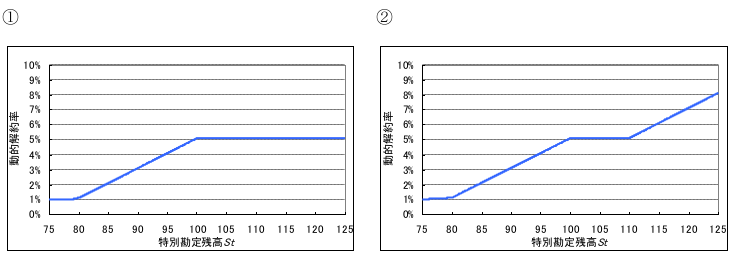
\includegraphics[scale=0.6]{images/ProbH24-1-2-2-1+2.png}\\
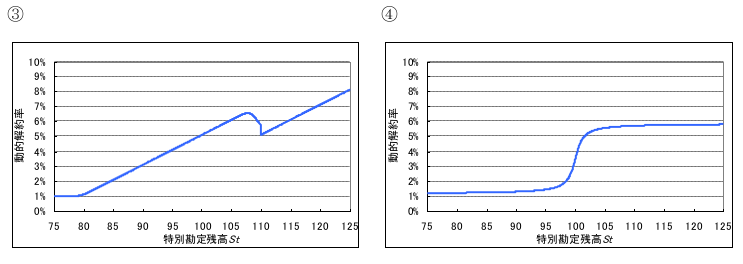
\includegraphics[scale=0.6]{images/ProbH24-1-2-2-3+4.png}\\
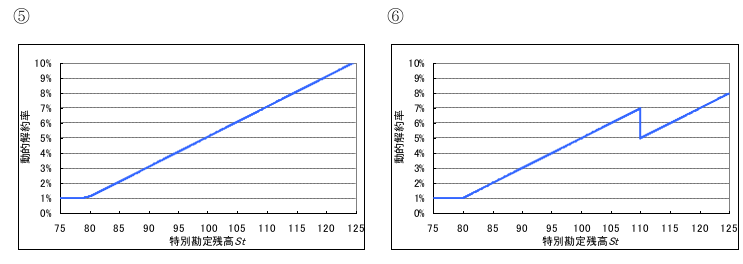
\includegraphics[scale=0.6]{images/ProbH24-1-2-2-5+6.png}

\answer{}
\noindent(ア)\\
選択肢:⑤\\
(選択した理由)

一般的に最低保証のある変額年金では、特別勘定資産残高が最低保証金額を下回っている
度合(インザマネーネス)が大きいほど解約率が低く、最低保証金額を上回っている度合
(アウトオブザマネーネス)が大きいほど解約率が高いと考えられる。ただし、解約返戻金
の最低保証がある場合には、上記のとおりになるとは限らない。
本問題において与えられた動的解約モデルの算式からは、最低保証金額は 100 で一定であ
る場合、動的解約率は $S_{t+1}$ の期待値に対して比例的に増加し、下限は 1.0\%である。
したがって、最も当てはまる選択肢は⑤である。\vspace{1zh} \\
(イ)\\
選択肢:③\\
(選択した理由)
(ア)と同様、一定額までは $S_t$が増加するにつれて解約率も上昇するが、110 に近づくに
つれてステップアップする確率が高まることにより解約率が減少。 $S_t$ が 110 以上の場合は、
最低保証金額は 110 から変動しないため、 $S_{t+1}$ の期待値の増加に対して比例的に増加する。
したがって、最も当てはまる選択肢は③である。\vspace{1zh} 

\noindent(補足)

上記解答例に記載したように、解約返戻金の最低保証がある場合には、特別勘定資産残高
が最低保証金額を下回っているからと言って、解約率が低くなるとは限らない。

本問題においては、解約返戻金の最低保証があるという設定になっており、この設定にお
いて、与えられた解約率のモデルが適切かどうかについては議論の余地があるが、本問題に
おいては、解約率のモデルは所与のものとなっており、このモデルに従うと、選択肢は一意
に定まる。

なお、採点にあたっては、上記の状況を考慮した。

\end{document}